\chapter{Predicting Stocks Using Sentiment Analysis - Felix} \label{ch:predictions_ml}
The movement of time series data for financial data is influenced by external effects. To leverage this we tried to add information from news sources to our trading strategies. For the hybrid prediction we estimate sentiment scores on news sources. This so called sentiment analysis is used to explore the orientation of the words or phrases in text data and their effect on the overall sentiment \citep{HADDI201326}. The original aim was to use financial news data to predict stock price movement and volatility for trading strategies. To achieve this, large amounts of text data would need to be preprocessed and analyzed regarding their connections to specific stocks, their topic and sentiment. The news data would need to be as precise as possible, because […] mention that an effect on the stocks an only be measured up to 20min after the news appear. Other sources say that… .
\\ \\
As we were not able to acquire access to a reliable and precise news sources, we tried to implement our approach on the available analyst reports regarding the ten specific stocks. The problem with these reports is, that they are more an indicator of performance over the past month and a prediction about the future performance. As such they do not cover sudden events that would be present in the news. The reports also cluster around certain dates with long stretches of no or very few reports in between (ABBILDUNG). This makes it unlikely that they are valuable for trading strategies.
%\begin{figure}[h]
%    \figuretitle{Seasonality in the Reports}
%    \centering
%    \begin{adjustbox}{width=.9\textwidth,center}
%    \input{figures/SeasonalityReports.png}
%    \end{adjustbox}  
 %   \caption{BLBLBLA}
 %   \label{fig:Seasonality in the Reports}
%\end{figure}{}
\\  \\
The goal was to identify the connection of specific articles to listed companies and compute a sentiment score for the article. There are many ways to calculate sentiment scores from flowing text data. Common procedures would be to use a library of previously known positive and negative adjectives or 4-grams. The simplest way to utilize these would be to simply count their appearance, this is known as a bag-of-words method (ZITAT?). Other approaches extract parts of the text at the location of the specific adjectives and use Support Vector Machines or Naive Bayes Classifier to extract sentiment, see \citet{westerski2007sentiment} for further references. Many of these more advanced sentiment classification techniques are supervised, as such they need a labelled data set for initial training. The 17153 analyst reports are unstructured and not labelled, making it unrealistic to use these methods. They also have a very specific format and language, therefore other pretrained models or other labelled training data sets could not be used. Another possibility to custom label the data would have been possible using intra day trading and news data. By looking at the movement or volatility of the period close after the news release approximate sentiment scores can then be computed \citep{robertson2007news}. As the obtained stock data is only inter day we could not apply this method.
%The analyst reports consist of scrapped text from reports that does nut necessarily follow a normal sentence like structure. This makes it difficult to apply syntactic based methods to extract adjectives from the flowing text based on semantic rules. 
\\ \\
Two methods to estimate sentiment scores in an unsupervised way will be explored here. One is a library bag-of-words approach that works with simple relative frequencies of positive and negative words. The other approach uses a new method called Joint Sentiment Topic model (JST) \citep{lin2009joint} and relies on a Bayesian method called Latent Dirichilet Allocation (LDA)  \citep{blei2003latent}. For both approaches the text data has to be cleaned which is described in section \ref{cleaningText}, the subsequent analysis of the sentiment scores can be found in section \ref{BoW} and \ref{JST}.

\subsection{Cleaning of the text data}\label{cleaningText}
To get reliable sentiment scores text data has to be preprocessed. The analyst reports contain 157380 unique words, characters and symbols. To improve the performance of unsupervised approaches good cleaning and reduction of dimensionality of the problem are important  \citep{HADDI201326}. The preprocessing was done in five steps using \texttt{R} \citep{Rproject}. At first words where converted to lowercase and all words where separated using the R package \textit{tidytext} \citep{tidytext}. Next all the stop words where removed by using a custom stop word library. Commonly stop word libraries from from the \textit{tidytext} package or others are being used. The problem with these libraries was that they contained a lot of sentiment adjectives that might be important for the extraction of reasonable sentiments. This reduces the total number of words from 67M initially to 43M, see figure \ref{fig:TotWord}. In the next step all links to websites, hyper-references, numbers, words with numbers and punctuation are removed as well. The result reduced the individual words and items from 157206 to 82525 by about 50 Percent. \\
\begin{figure}[h]
\centering
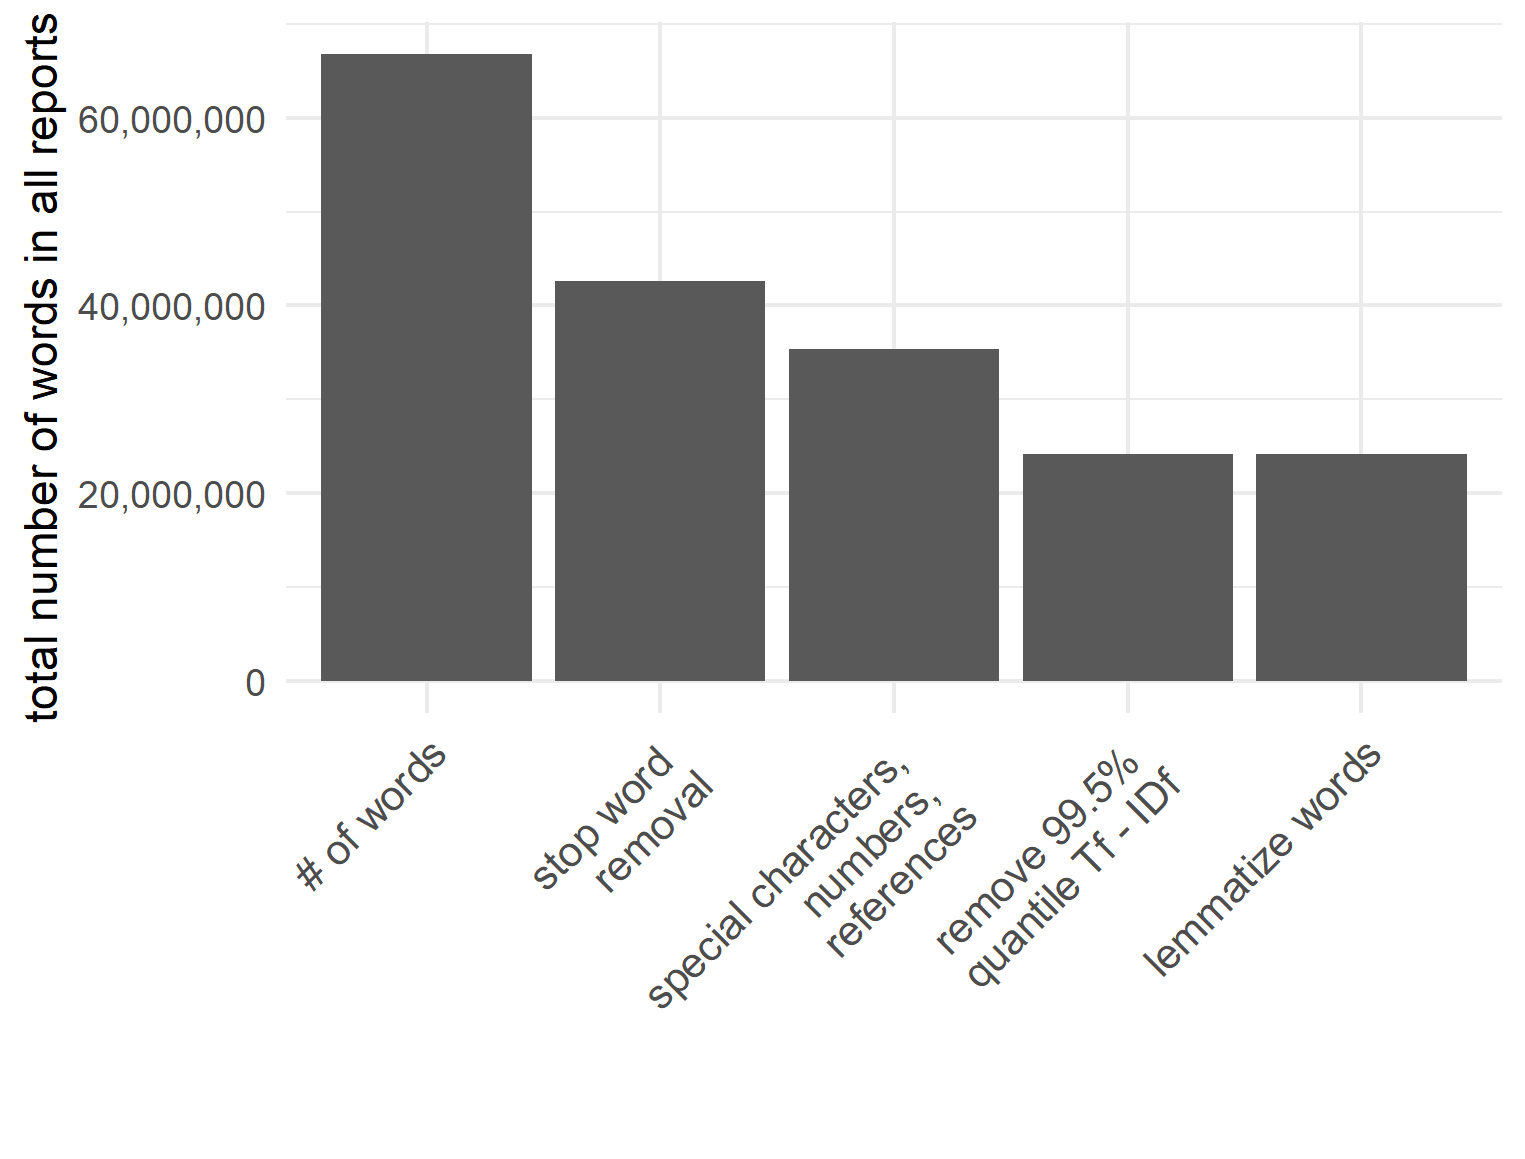
\includegraphics[width=\textwidth]{figures/ReductionInTotalNWords.png}
\caption{Reduction in total number of words due to preprocessing the data.}
\label{fig:TotWord}
\end{figure}

A common way to look at feature importance in flowing text data is to look at the Term Frequency Inverse Document Frequency (TF-IDF) which puts the feature frequency (FF) also called term frequency (TF) in relation to the inverse document frequency (IDF) \citep{na2004effectiveness}. 
\begin{equation}
    TF-IDF = FF * Log(\frac{N}{DF})
\end{equation} 
Where N represents the number of documents and is DF the number of documents that contain this feature, calculated as the sum of the feature presence (FP). The result is a probability between 0 and 1 for each word. For a large number of words, as in our case, TF-IDF values are usually quite low. For topic modelling like LDA the lower 10 Percent of words are often removed, because they contain relatively frequent words over all documents. Here we are doing the opposite. Due to the structure of the data of ten different stocks and company specific reports we want to avoid fitting company specific topics in the JST model. Removing the 99.5 Percent upper quantile of TF-IDF words seemed to improve the performance. Leaving just over 24M words in total. This represents the removal of an additional 10293 individual words. The fifth and last step is lemmatizing the words using the \textit{textstem} package \citep{textstem}. Lemmatizing words means reducing them to their inflectional forms. We did not stem the words because it sometimes changes the meaning of words, which is important for sentiment analysis. \\ \\

After these five cleaning steps the number of individual words and items was reduced from 157380 to 64228 by about 60 Percent and of the total number of words only 36 Percent are left. The summary statistics for the total number of words in each report in table \ref{tab:summaryCR} show the result more clearly. 
\begin{table}[ht]
\centering
\begin{tabular}{rllllll}
  \hline
  & Min. & 1st Qu. & Median  &  Mean & 3rd Qu. &   Max. \\
  \hline
  original reports & 16  &  1913  &  3230 &   3834  &  4785  & 21502  \\ 
  cleaned reports  & 0   &  729  &  1232  &  1400  &  1803  &  7218  \\ 
   \hline
\end{tabular}\label{tab:summaryCR}
\caption{Summary statistics for the number of words in each report}
\end{table}

%After validating the cleaned text different uncleaned items, like words consisting of multiples of the same letter, where discovered. We did not find a way to remove them.

\subsection{Sentiment Library}\label{BoW}
The simplest approach for estimating unsupervised sentiment scores is applying a library of as positive and negative defined words to the data. The resulting polarity towards positive or negative sentiment can then be achieved by calculating relative probabilities
\begin{equation}
    Polarity = \frac{P - N}{P + N}
\end{equation}
of the sum of positive words (P) and negative words (N). Some more advanced libraries even weight the appearance of each word, but we could not find any stock and financial news specific library that does that. Instead we used a library from \citet{sent_dictionary} as simple word list. An excerpt from the list can be found in table \ref{tab:sent_dic}. 
% latex table generated in R 3.6.0 by xtable 1.8-4 package
% Sun Sep 08 17:25:29 2019
\begin{table}[ht]
\centering
\begin{tabular}{rll}
  \hline
 & positive & negative \\ 
 & $n = 218$ & $n = 1282$ \\ 
  \hline
  1 & acclaim & abandonment \\ 
  2 & accomplishment & abdication \\ 
  3 & advantage & abuse \\ 
  4 & assure & acquittal \\ 
  5 & attractiveness & catastrophe \\ 
  6 & delightful & criticize \\ 
  7 & diligent & degrade \\ 
  8 & impress & harsh \\ 
  9 & \vdots & \vdots \\ 
   \hline
\end{tabular}\label{tab:sent_dic}
\caption{Excerpt from the sentiment dictionary by \citet{sent_dictionary}}
\end{table}
The results of applying the sentiment library to the reports can be found in figure \ref{fig:BoWSentiment}. The histogram shows an approximate normal distribution around zero. This also means the the imbalance in the number of positive ($n = 218$) and negative ($n = 1282)$) words seems to be about right.
\begin{figure}[h]
\centering
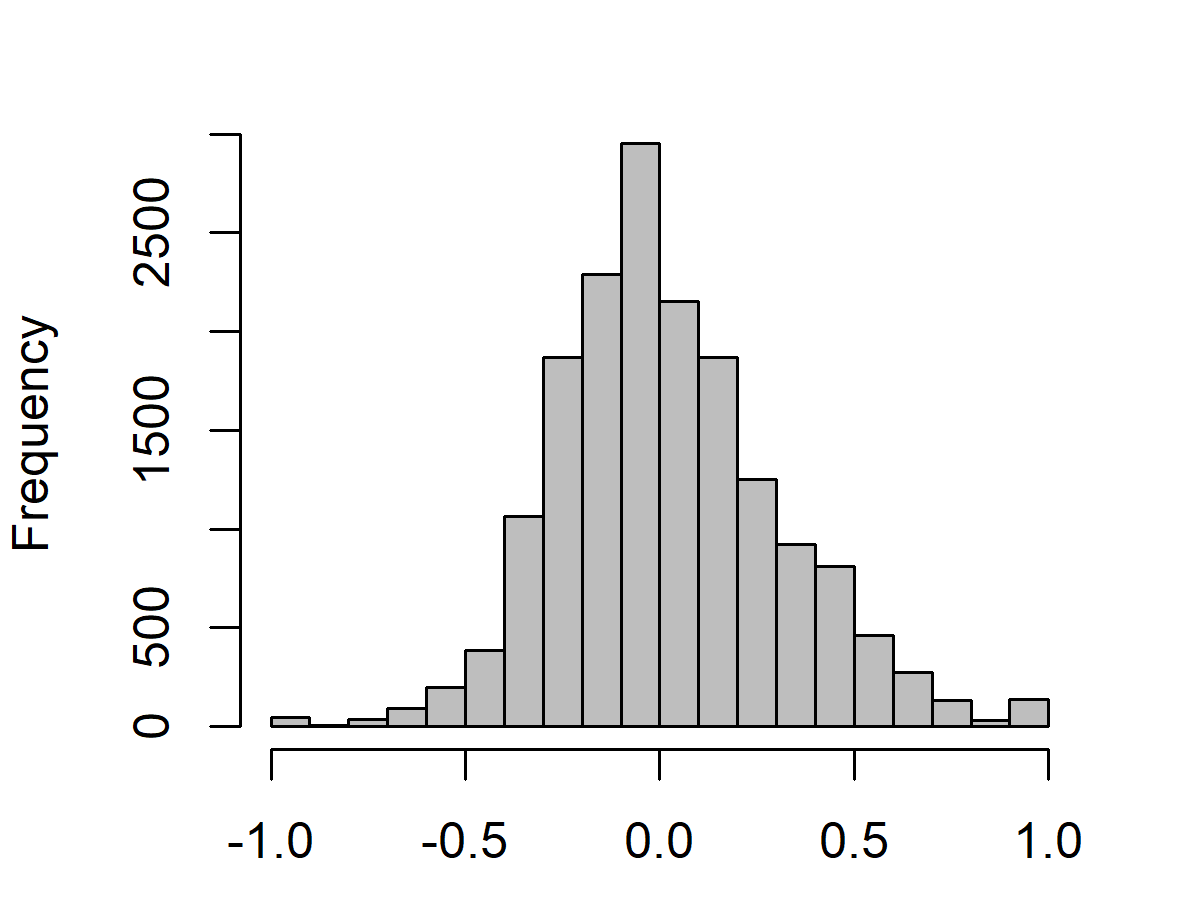
\includegraphics[width=4in]{figures/2SentimentsBOW_Histogram.png}
\caption{Histogram of the sentiment scores computed by the sentiment library}
\label{fig:BoWSentiment}
\end{figure}



\subsection{Joint sentiment topic model}\label{JST}
To make the computation of the sentiment scores more adaptable to the specific format of the data a new method by \citet{lin2009joint} called Joint Sentiment Topic model (JST) is being used. This approach builds upon the idea of \citet{blei2003latent} to use a Bayesian hierarchical model, called Latent Dirichilet Allocation (LDA), to compute topics from text data. Latend Dirichilet Allocation is one of the most sophisticated methods in the field of topic modelling. To understand JST we firstly explain the fundamentals and assumptions of LDA. \\ 

% good video: https://www.youtube.com/watch?v=DWJYZq_fQ2A
The general idea of LDA is that each document can be described by a distribution of topics and each topic can itself be described by a distribution of words \citep{blei2003latent}. This assumes that the words themselves are independent of each other which is in reality not the case, but for large data sets this assumption seems to be acceptable. To train a LDA one decides on the number of topics ($T$) that occur within the text documents and have not been observed, they are latent. The LDA has two dirichilet priors containing hyperparameters $\alpha$ and $\beta$, a high $\alpha$ indicates that each document is likely to contain a mixture of many topics, similarly a high $\beta$ indicates that each topic is a mixture of many different words. LDA backtracks from the document level to identify topics that are likely to have generated this specific corpus of words. The underlying optimisation of the model is done using a Gibbs-Sampler. In the first step, each word is assigned probabilities to belong to each of the $T$ topics that sum up to one and each document gets a probability for each topic. The algorithm then iterates over the words topics and documents, updating the underlying probabilities. \\ \\
In the JST the LDA is extended from three hierarchical layers to four. The additional layer determines the document sentiment by adding a layer in between the document and topic layer \citep{lin2009joint}. The new sentiment layer can be associated with documents, followed by topics and then words. For a detailed mathematical definition see \citet{lin2009joint}. \\ \\
To estimate the JST models we used the \textit{rJST} package in R \citep{rJST} and added the sentiment dictionary from the previous section \ref{BoW} as prior information for performance improvements.

The output are posterior probabilities for sentiments and topics of each document, as well as the posterior probabilities of each word loading onto topics. For a large and diverse enough training data set the returned posterior probabilities of the words can be used to determine the topics and sentiment in new documents. The JST therefore does not need to be retrained at each new observation. \\ \\

The results of the JST model need to be evaluated if the results split the data in reasonable topics and associated sentiments. Because we do not have any labelled training data we cannot check the convergence of the model with classical accuracy scores used in \citet{lin2009joint}. Instead we examine the highest loading words per sentiment and topic and the distribution of the sentiment scores. Due to the fact that we only have analyst reports for ten different stocks the results of the JST can at least be questioned. During the training of different models and experimenting with different data preparation steps the model often indicated splitting the data on special stock specific topics, instead of general topics associated with sentiments. Improvements where achieved by using a custom stop word dictionary that only contains few adjectives and the removal of the 99.5 Percent quantile of the TF-IDF words. We decided on using the JST model with 30 topics by comparing the results of models with 10, 20, 30 and 50 topics for different learning rates and numbers of iteration, because it returned the most reliable results. \\

Table \ref{tab:tab:postProbSent1} gives an overview over the words  with the highest posterior probability for sentiment one on topic one to three and thirty (see appendix for Table sentiment two \ref{tab:postProbSent2} ). It is still visible that the documents are from a business context but words indicating the sentiment like good, growth, high are only few. This makes it hard to tell if sentiment one is positive, negative or even something different. \\
% latex table generated in R 3.6.0 by xtable 1.8-4 package
% Fri Sep 13 15:15:05 2019
\begin{table}[ht]
\centering
\begin{tabular}{rllll}
  \hline
 & topic1sent1 & topic2sent1 & topic3sent1 & topic30sent1 \\ 
  \hline
1 & good & year & customer & price \\ 
  2 & look & margin & year & volatility \\ 
  3 & company & will & service & day \\ 
  4 & just & good & will & stock \\ 
  5 & question & growth & business & financial \\ 
  6 & mean & market & believe & average \\ 
  7 & make & expect & continue & expect \\ 
  8 & want & service & datum & year \\ 
  9 & right & continue & growth & next \\ 
  10 & business & high & line & group \\ 
  11 & talk & next & fix & express \\ 
  12 & people & single & also & report \\ 
  13 & time & still & price & month \\ 
  14 & content & also & industry & rate \\ 
  15 & without & digit & time & person \\ 
   \hline
\end{tabular}\label{tab:postProbSent1}
\end{table}
Another way to evaluate the model is to take a closer look at the posterior probabilities for the sentiments. The histogram in figure \ref{fig:JSTSentiment} displays a reasonable split done by the sentiments. As we computed only positive and negative sentiment scores and left out a neutral class the histogram for sentiment two is this one flipped. The calculated sentiments also seem to lean towards the left. This might indicate that sentiment two was the more prominent one in the data. \\
\begin{figure}[h]
\centering
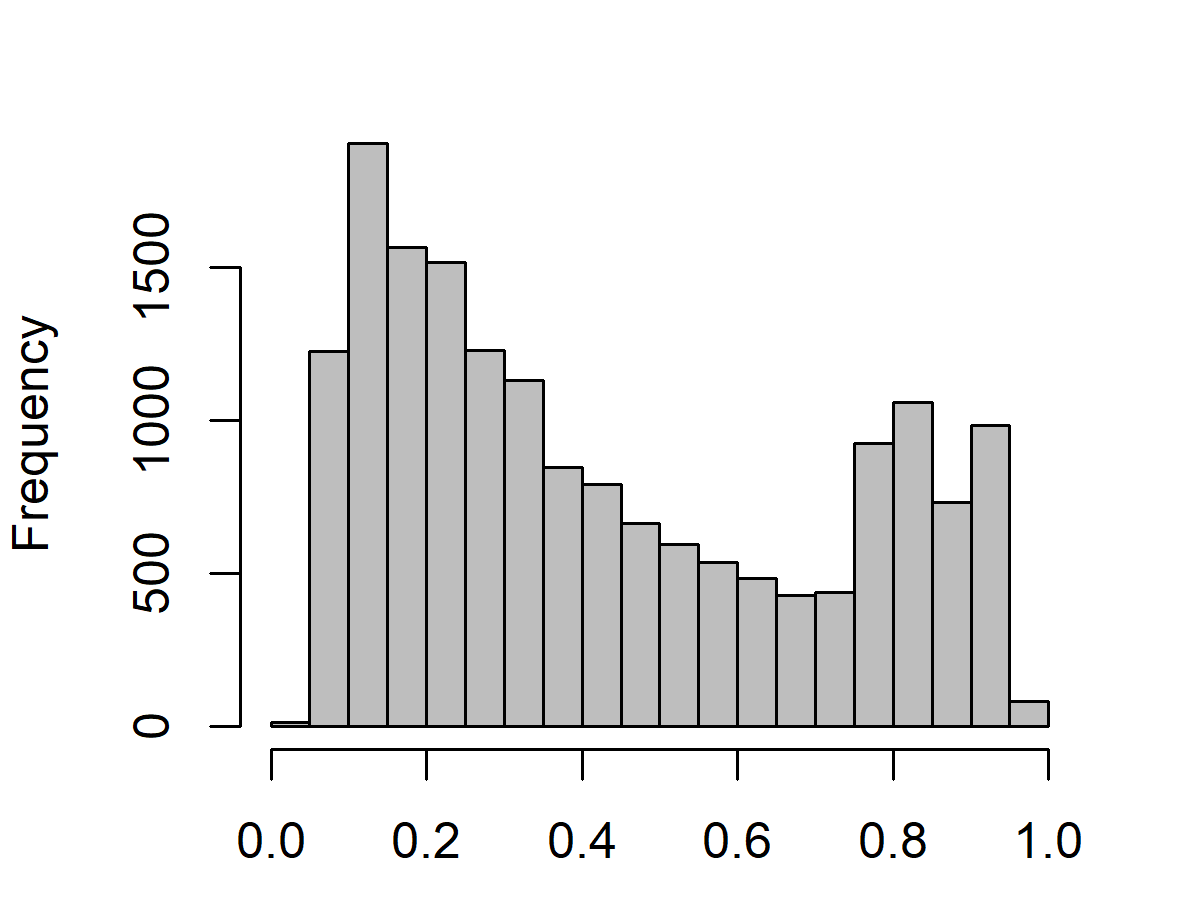
\includegraphics[width=4in]{figures/2SentimentsJST_Histogram.png}
\caption{Histogram of the sentiment scores computed by the Joined Sentiment Topic model}
\label{fig:JSTSentiment}
\end{figure}
The results of the unsupervised Joint Sentiment Models are difficult to evaluate and we have to be at least wary of the results we obtained. Problematic in this case could also be, that the JST views the documents as bag of words and therefore also ignores the ordering of words. Business language contains a lot of fixed phrases that are not considered here.  Nonetheless they might be an informative feature for the estimation of stock price movements in the next section. 


\subsection{XG-Boost on sentiment data}
Based on the RavenPack data and our own custom sentiment scores we tried to make predictions for the movement of the time series of different stocks. Inspired by different Kaggle competitions and \citep{li2018predicting} we decided to try using XGBoost for binary classification of upwards of downwards movement. For continuous predictions, considering the time dependent structure see section ??????. Here the special time dependent structure of the time series is mostly disregarded and instead a gradient tree boosting algorithm called XGBoost will be used. A additional benefit of doing this is the identification if our sentiment scores or the ones from RavenPack are useful in predicting the movement. \\

XGBoost is a gradient tree boosting method developed by \citet{Chen_2016} and has several beneficial properties. Next to the computational properties it scales well for large data sets and can handle missing values internally. A possible competitor would be LightGBM by \citet{Ke2017LightGBMAH} from Microsoft. The general idea behind tree boosting is that they split data it leaf wise with the best fit, whereas other boosting algorithms split the tree level wise. This means splits are done only at the position where the loss can be reduced the most. Each model consists of a predefined number of trees trying to complement each other with a set of classification and regression trees (CART). The tree ensemble method was originally developed by \citet{friedman2001greedy} and XGBoost which stands for \enquote{Extreme Gradient Boosting} can be seen as an extension of the framework. Most of the improvements where done in finding the optimal split at each level, leaf of the tree, because enumerating over all possible solutions is usually computationally impossible. 
% good explanation: https://xgboost.readthedocs.io/en/latest/index.html
% mehr mathe?
Missing values are handled internally by XGBoost \citep{Chen_2016}. The model learns automatically where to go when a value is missing. For a large enough amount of data this is similar to imputing a value but based on a reduction on training loss. 

\begin{itemize}
    \item How we engineered the fatures
    \item XGB kann auch einfach nur verwendet werden um zu erkennen welche features wichtig sind
    \item under normal conditions we would need to retrain the model after each prediction but as we are usind the log returns which are similar to a random walk this isn´t really necessary. 
    %https://towardsdatascience.com/3-facts-about-time-series-forecasting-that-surprise-experienced-machine-learning-practitioners-69c18ee89387
    \item What we did not try but what would be interesting is: They take this idea a step further in Financial Time series modelling, where they actually have classes of models built explicitly for modeling the uncertainty of a time series, as opposed to the time series itself, such as ARCH and GARCH models.
    \plots how to select optimal XGboost parameters:
    https://towardsdatascience.com/selecting-optimal-parameters-for-xgboost-model-training-c7cd9ed5e45e
    \item paramter tuning xgBoost
    % https://www.analyticsvidhya.com/blog/2016/03/complete-guide-parameter-tuning-xgboost-with-codes-python/
    \item GB-Tree methods have problems with trends:
    % https://medium.com/datadriveninvestor/why-wont-time-series-data-and-random-forests-work-very-well-together-3c9f7b271631
    \item Missing value handling: Internally, XGBoost will automatically learn what is the best direction to go when a value is missing. Equivalently, this can be viewed as automatically "learn" what is the best imputation value for missing values based on reduction on training loss.
    \item the story behind XGB: https://homes.cs.washington.edu/~tqchen/2016/03/10/story-and-lessons-behind-the-evolution-of-xgboost.html
    
\end{itemize}
\subsubsection{XGBoost}
Here I expalain what XGBoost is an how it works

\subsection{Classification results}
Take Mean of different predictions?

XGBOOST, LightGBM whatever. 
Theorie, Datenaufbereitung, Ergebnisse

The standard evaluation of binary classification results is done using the F1-measure \citep{HADDI201326}. Where the score is a weighted product of precision and recall
\begin{equation} 
    F-measure = \frac{2*precision * recall}{precision + recall}
\end{equation}

% https://www.kaggle.com/furiousx7/xgboost-time-series
% related literature at the end
% Hourly forecasting: https://www.kaggle.com/robikscube/tutorial-time-series-forecasting-with-xgboost/notebook
% https://www.datacamp.com/community/tutorials/xgboost-in-python
% missing values in XGB https://github.com/dmlc/xgboost/issues/21


